\begin{appendices}

\chapter{Fichiers LQL Nagios}
\label{annexe:fichiersLQLNagios}

Cette annexe permet une vue sur les fichiers LQL permettant la r\'ecup\'eration des informations de Nagios. 
Ces informations sont ensuite trait\'ees par le service Web qui se charge de remplir ou actualiser la base de donn\'ees en cons\'equence.

\subsubsection{R\'ecup\'eration des salles}

La requ\^ete~\ref{annexe:nagiosGetHostGroups} permet de r\'ecup\'erer les salles que Nagios surveille.
Ces salles sont appel\'ees \textit{hostgroups} et contiennent des machines appel\'ees \textit{hosts}.
Parmi ces \textit{hostgroups}, les imprimantes, serveurs et autres ressources sont exclues pour ne retenir que les salles.
La socket Nagios retournera alors le nom de la salle, le nombre de machines qu'elle contient, et la liste des machines qui font partie du groupe.

\vspace{0.20cm}

\lstinputlisting[language=LQL]{codes/nagiosGetHostGroups.ngs}
\captionof{figure}{Code LQL de r\'ecup\'eration des salles que surveille Nagios}
\label{annexe:nagiosGetHostGroups}

\subsubsection{R\'ecup\'eration des machines}

La requ\^ete~\ref{annexe:nagiosGetResources} permet de r\'ecup\'erer toutes les machines qui peuvent poss\'eder un utilisateur de connect\'e.
En fait, il est demand\'e la r\'ecup\'eration de tous les services ayant acc\`es \`a l'information \textsf{check\_whoisloggedin}, donc qui est connect\'e actuellement.
Il y a pour chaque machine, un service portant ce nom, cela revient donc \`a demander tous les ordinateurs.
La socket Nagios retournera alors le nom de la machine, son adresse IP, le \textsf{host\_groups} donc le nom de la salle \`a laquelle elle appartient, son \'etat et enfin l'utilisateur connect\'e s'il y en a un.

\clearpage

\lstinputlisting[language=LQL]{codes/nagiosGetResources.ngs}
\captionof{figure}{Code LQL de r\'ecup\'eration des machines que surveille Nagios}
\label{annexe:nagiosGetResources}

\subsubsection{R\'ecup\'eration de tous les utilisateurs connect\'es}

La requ\^ete~\ref{annexe:nagiosGetUsersLogged} permet de r\'ecup\'erer seulement la liste des utilisateurs connect\'es sur les machines sous surveillance.
Il est demand\'e la r\'ecup\'eration de tous les services parmi lesquels il n'est gard\'e que ceux qui peuvent avoir un utilisateur de connect\'e.
De plus, les messages de Nagios concernant un \'eventuel probl\`eme dans la r\'ecup\'eration de l'information sont \'ecart\'es.
Seul les utilisateurs \og corrects\fg{} sont gard\'es.

\vspace{0.20cm}

\lstinputlisting[language=LQL]{codes/nagiosGetUsersLogged.ngs}
\captionof{figure}{Code LQL de r\'ecup\'eration des utilisateurs connect\'es sur les machines que surveille Nagios}
\label{annexe:nagiosGetUsersLogged}

\chapter{Retour de requ\^ete LQL}
\label{annexe:reponseLQLNagios}

Cette annexe permet une vue sur les informations qui sont retourn\'ees par une requ\^ete LQL.
Les informations se pr\'esentent toujours sous la m\^eme forme : une ligne est compos\'e des diff\'erentes colonnes demand\'ees dans la requ\^etes.
Les colonnes sont s\'epar\'ees par un \textsf{; (point-virgule)}.

\subsubsection{Retour lors d'une r\'ecup\'eration des salles}

La r\'eponse~\ref{annexe:reponseNagiosGetHostGroups} correspond \`a l'ex\'ecution de la requ\^ete~\ref{annexe:nagiosGetHostGroups} sur le serveur contenant Nagios.

\begin{figure}[!ht]
	\centering
	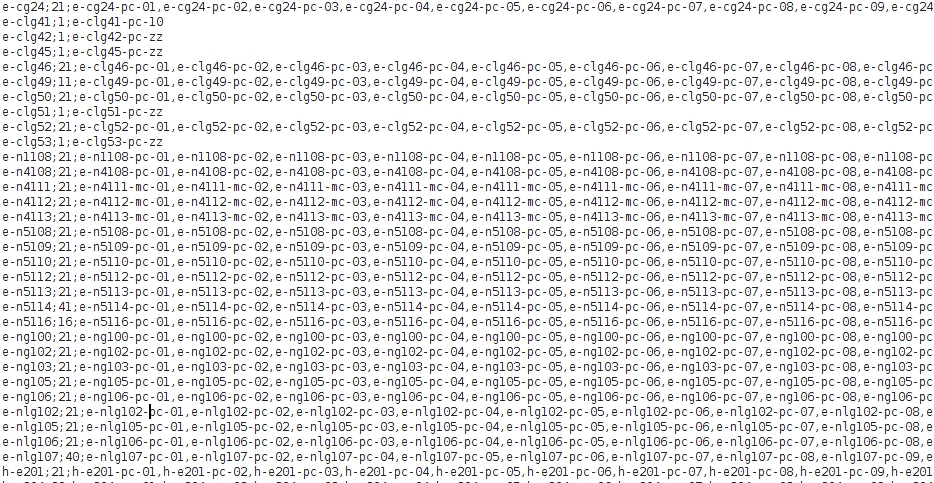
\includegraphics[scale=0.45]{reponseNagiosGetHostGroups.jpg}
	\caption{R\'eponse lors d'une requ\^ete de r\'ecup\'eration de salle}
	\label{annexe:reponseNagiosGetHostGroups}

\end{figure}

\subsubsection{Retour lors d'une r\'ecup\'eration des machines}

La r\'eponse~\ref{annexe:reponseNagiosGetResources} correspond \`a l'ex\'ecution de la requ\^ete~\ref{annexe:nagiosGetResources} sur le serveur contenant Nagios.

\begin{figure}[!ht]
	\centering
	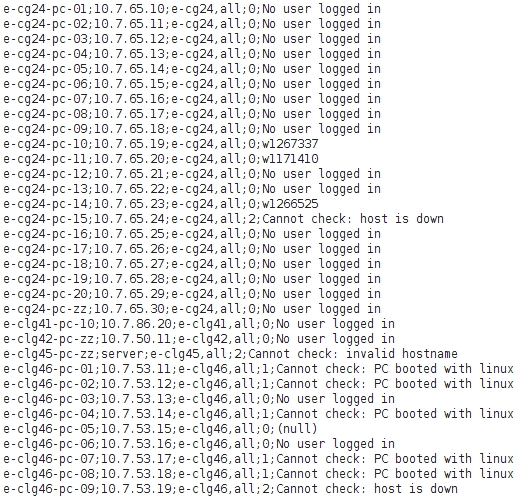
\includegraphics[scale=0.5]{reponseNagiosGetResources.jpg}
	\caption{R\'eponse lors d'une requ\^ete de r\'ecup\'eration des machines}
	\label{annexe:reponseNagiosGetResources}

\end{figure}

\subsubsection{Retour lors d'une r\'ecup\'eration des utilisateurs}

La r\'eponse~\ref{annexe:reponseNagiosGetUsersLogged} correspond \`a l'ex\'ecution de la requ\^ete~\ref{annexe:nagiosGetUsersLogged} sur le serveur contenant Nagios.

\begin{figure}[!ht]
	\centering
	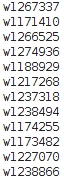
\includegraphics[scale=0.5]{reponseNagiosGetUsersLogged.jpg}
	\caption{R\'eponse lors d'une requ\^ete de r\'ecup\'eration des utilisateurs}
	\label{annexe:reponseNagiosGetUsersLogged}

\end{figure}

\end{appendices}

\clearpage
